\section{Гиперпараметры. Задача настройки гиперпараметров. Связь с задачей выбора алгоритма.}

\D{
    Гиперпараметры =
    \begin{itemize}
        \item Параметры алгоритма обучения
        \item (Параметры, не меняющиеся во время обучения)
    \end{itemize}
}

\D{
    Задача настройки гиперпараметров
    \begin{itemize}
        \item D = набор данных
        \item A = алгоритм обучения
        \item p = гиперпараметры
        \item L = функция ошибки
    \end{itemize}

    Найти $p_{best} = \arg \min_p L(A(p), D)$
}


\begin{figure}[H]
    \centering
    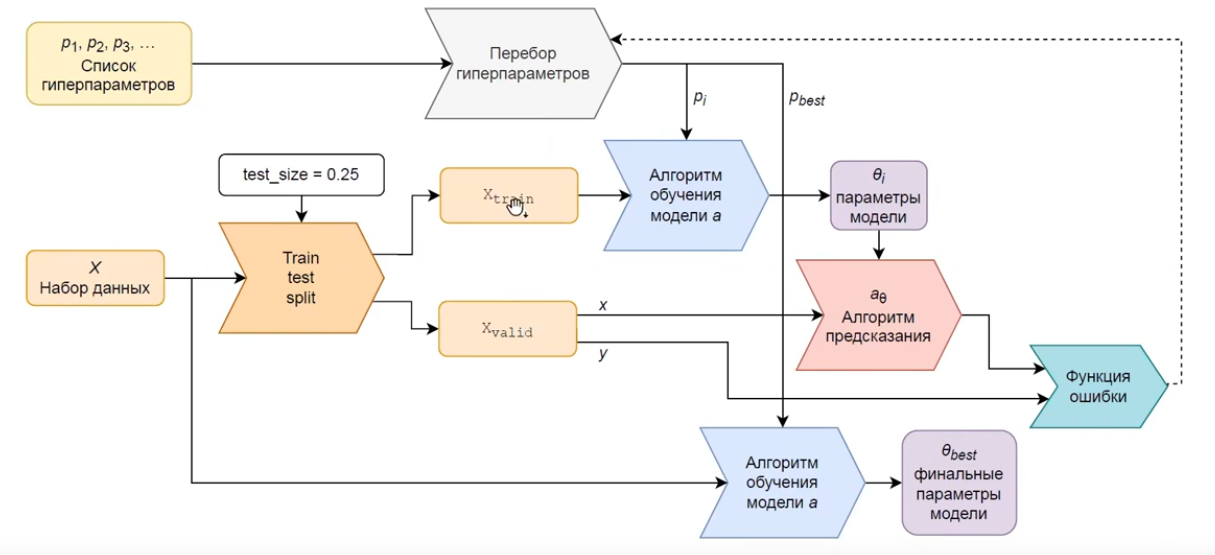
\includegraphics[scale=.4]{images/hp_train}
    \caption{Подбор гиперпараметров в процессе обучения}
\end{figure}

Функция ошибки также может быть гиперпараметром, но при этом
потребуется внешняя функция ошибки.

Связь с задачей выбора алгоритма: можно рассматривать гиперпараметры
как параметры алгоритма обучения и решать задачу выбора алгоритма
на алгоритмах обучения с различными фиксированными гиперпараметрами.

\T{
    Задачу выбора алгоритма можно свести к задаче настройки
    гиперпараметров.

    \begin{proof}
        Рассмотрим несколько алгоритмов: $A^1, A^2 ...$ с
        соответсвующими множествами гиперпараметров $\{p_1^1, p_2^1, ...\}, ...$

        Построим универсальный алгоритм $A^u$ со списком гиперпараметров
        $\{c, p_1^1, ..., p_1^2, ...\}$, где $c$ указывает на
        выбираемый алгоритм $A^c$

        Теперь задача выбора алгоритма и гиперпараметров решается
        как задача подбора гиперпараметров универсального алгоритма.
    \end{proof}
}

\T{
    Настройка гиперпараметров $\to$ выбор алгоритма.

    \begin{proof}
        Зафиксируем все возможные комбинации гиперпараметров
        и построим по ним уникальные алгоритмы.

        Затем решаем задачу выбора алгоритма.
    \end{proof}
}

Разделить задачи можно по типу:
\begin{itemize}
    \item Категориальные гиперпараметры можно назвать алгоритмами
    \item Числовые оставить гиперпараметрами
\end{itemize}



% \begin{figure}[H]
% 	\centering
% 	\begin{minipage}[b]{0.4\textwidth}
% 		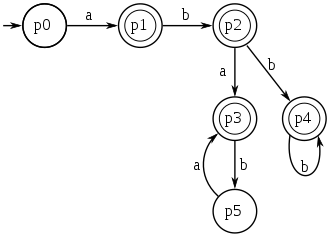
\includegraphics[width=\textwidth]{images/dfa.png}
% 		\caption{Пример графа переходов детерминированного КА.}
% 	\end{minipage}
% 	\hfill
% 	\begin{minipage}[b]{0.4\textwidth}
% 		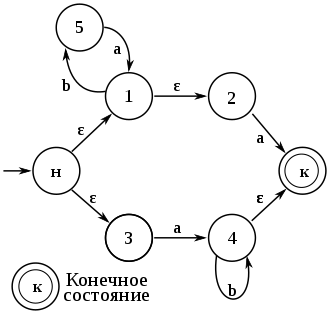
\includegraphics[width=\textwidth]{images/ndfa.png}
% 		\caption{Пример графа переходов недетерминированного КА с самопроизвольными переходами.}
% 	\end{minipage}
% \end{figure}